% !Mode:: "TeX:UTF-8"
\chapter{非凸优化与深度学习基本理论}
\label{chap:theory}

\section{引言}
非凸优化理论在低秩矩阵分解或补全、盲反卷积、字典学习、深度学习和相位恢复领域有着广泛而深刻的应用,是国内外学者研究的热点。相较于凸优化理论中凸问题、输入样本和优化算法的完备性,非凸化理论存在诸多难题未被完美解决。但是某些非凸问题在实践应用中有着高效的求解算法和严格的收敛性分析。在非凸统计模型(包括低秩矩阵补全、盲反卷积与相位恢复)中,因为经验损失一般为非凸函数,有效的求解算法需要正则化保证梯度下降算法快速收敛。一般优化算法例如梯度下降需要合适的学习率避免迭代过程中偏离最优解,但是算法的收敛性却无法保证。非凸统计模型暗含隐式的正则化先验,此时梯度下降算法遵循隐式正则化提供的修正梯度方向收敛到与梯度随机采样机制无关的最优解邻域。神经网络的训练主要通过求解经验损失函数或结构化损失函数来完成,但这是一个困难的非线性优化问题,传统的优化理论难以直接应用。在神经网络和优化的交叉领域,长期以来研究人员积累了大量的理论研究和知识,不过这些研究或过于理论而不被大部分实践者所了解,或过于偏工程而不被理论学者所理解和欣赏。

近年来图像处理领域的研究表明,深度学习技术可以有效解决线性图像反问题,包括图像去噪、核磁共振成像和图像超分辨率。深度残差网络DnCNN与IRCNN模型学习高斯噪声分布,其去噪性能一度超越了传统的BM3D算法。上述监督学习算法需要大量的清晰图像与含噪图像对训练残差网络,基于无监督学习的深度图像先验方法利用解码-编码网络本身暗含的图像先验知识可有效去除噪声。由此表明,深度学习领域的观点和方法可迁移至解决图像处理领域,有关深度图像先验应用于非线性图像反问题中的相位恢复问题有待进学者一步研究。

\section{非凸优化的基本问题与优化算法}
优化领域最大的分野是凸与非凸,并非线性与非线性。凸优化研究在凸集上最小化凸函数的问题,大量关于凸优化的研究已经为许多类凸问题提出了有效的求解算法。因此,凸优化已经广泛地影响了科学和工程的各个学科\supercite{Stephen3}。

近年来,凸优化算法彻底改变了离散和连续优化问题的算法设计。对于子模函数最小化、整数规划和图的最大流等问题,已知的最快算法涉及到对凸优化算法的基本理论的重要应用,如梯度下降法、镜像下降法、内点方法和切割平面方法\supercite{Stephen1,Stephen2,Stephen3,Goldstein,Heide,Thomas,Chambolle1,Martin}。机器学习中的大规模优化问题对凸优化算法的需求也极大地推动了凸优化技术本身的发展。一般的凸优化问题如下所示:
\begin{equation} \label{problem:2-1}
	\begin{aligned}
		&\text{minimize}\quad f_{0}(x) \\
		&\begin{array}{@{}l@{\quad}l@{\quad}l@{}}
			\text{subject\ to}
			&f_{i}(x)\leq 0, &i=1,\ldots,m \\
			&h_{i}(x)=0, &i=1,\ldots,p \\
		\end{array}
	\end{aligned}
\end{equation}
其中$x\in\mathbb{R}^n$表示优化变量,$f_{0}(x)$表示目标函数,$f_{i}(x)\leq{0}$表示不等式约束,$h_{i}=0$表示等式约束。若$f_{0},f_{1},\ldots,f_{m}$为凸函数,$h_{i}=0$为仿射集,则式\eqref{problem:2-1}为标准的凸问题。此外,凸优化问题具有以下方面的优势:(1)凸优化问题的局部最优解就是全局最优解;(2)某些非凸问题可以通过凸松弛技术转化为凸优化问题或者近似为凸优化问题(例如拉格朗日对偶问题);(3)凸优化问题的研究较为成熟,当一个优化问题具体被归纳为一个凸优化问题时,基本可以确定该问题是可被求解的。本章基于Pytorch框架实现了凸优化算法包,其地址见\url{https://github.com/chaidisheng/Convex_Optimization}。

较之于凸优化问题,一般非凸优化问题包括三类:优化变量离散、可行集非凸或代价函数非凸\supercite{Chambolle2,Andreas,Xu,Fengmiao,PanShaohua,SunTao}。非凸优化是机器学习等领域中的基本问题,迭代优化方法缺乏理论支撑\supercite{PanShaohua, SunTao}。基于这个原因,一些学者一直致力于非凸优化理论方面的研究\supercite{SunTao,Chi,Liu,Ruoyu,Cong,Xiangyi,Danilova,Dongruo}。以下将介绍非凸优理论中基本的非凸问题与优化算法。
\subsection{主要概念}
\begin{definition} \label{def:2.1}
	凸函数:一个函数$f$被称为凸函数,如果对任意$x,y$,满足
	\begin{equation} 
		f(y)\geq{f(x)+\left\langle{\nabla f(x), y-x}\right\rangle}.
	\end{equation}
	或者对任意$x,y,0\leq\theta\leq1$,满足
	\begin{equation} 
		f(\theta x + (1-\theta)y)\leq\theta f(x)+(1-\theta)f(y).
	\end{equation}
\end{definition}

\begin{definition} \label{def:2.2}
	强凸性:一个函数$f$被称为$\mu-$强凸函数,如果对任意$x,y$,满足
	\begin{equation}
		f(y) \geq f(x)+\left\langle{\nabla f(x), y-x}\right\rangle +\frac{\mu}{2}\Vert y - x \Vert^{2}.
	\end{equation}
\end{definition}	

\begin{definition} \label{def:2.3}
	利普希茨连续性:一个函数被称为是$L_{f}$-Lipschitz,如果对任意$x,y$,满足
	\begin{equation}
		\Vert f(x) - f(y)\Vert \leq L_{f}\Vert x - y\Vert.
	\end{equation}
	另一个等价的条件为:
	\begin{equation}
		\Vert g \Vert \leq L_{f},\;g\in \partial f(x). 
	\end{equation}
\end{definition}
	
\begin{definition} \label{def:2.4}
	光滑性:一个函数$f$被称为$L_{g}$光滑(梯度是$L_{g}$-Lipschitz),如果对任意$x,y$,满足
	\begin{equation}
			\Vert  \nabla f(x) - \nabla f(y)\Vert \leq L_{g}\Vert x - y\Vert.
	\end{equation}
	或者
	\begin{equation}
		f(y) \leq f(x)+\left\langle{\nabla f(x), y-x}\right\rangle +\frac{L_{g}}{2}\Vert y - x \Vert^{2}.
	\end{equation}
\end{definition}

\begin{definition} \label{def:2.5}
	单调算子:在$\mathbb{R}^n$上的算子$F$称为单调算子,如果对$\forall(x,u),(y,v)\in{F}$,满足
	\begin{equation}
		(u-v)^\top(x-y)\geq{0}.
	\end{equation}
%	若$f(x)$为闭凸函数(Convex Closed Proper,CCP),则$F(x)=\partial{F(x)}$为最大单调算子。
\end{definition}

\subsection{基本的非凸问题}
广泛的科学与工程应用问题其本质在于求解非线性方程组\supercite{Cong}。给定观测数据$y=\left\lbrace y_{j} \right\rbrace_{1\leq j\leq m}$,它对应的非线性系统为
\begin{equation} \label{equation:2-1}
	y_{j}\approx \mathcal{A}_{j}(x),\quad 1\leq j \leq m,
\end{equation}
其中$x\in\mathbb{R}^n$表示系统输入,$\mathcal{A}_{j}$表示非线性映射。如何设计重构$x$的高效优化算法是低秩矩阵补全、相位恢复、神经网络训练等信息与统计科学领域亟待解决的难题\supercite{PanShaohua,Ruoyu,Cong,Danilova}。在合理的高斯噪声容限下,式\eqref{equation:2-1}转化为经验损失最小化问题:
\begin{equation} \label{problem:2-2}
	\mathop{\text{minimize}}\limits_{x\in\mathbb{R}^n}\quad f(x)=\sum_{j=1}^{m}|y_{j}-\mathcal{A}_{j}(x)|^{2}.
\end{equation}
一般地,优化问题\eqref{problem:2-2}非凸且属于NP难问题,难以在多项式时间复杂度内求解。工程应用中,非线性系统优化问题可用式\eqref{problem:2-2}统一表示。以下阐述几个基本的非凸优化问题:

(1)相位恢复问题:假设给定编码衍射模型传输矩阵的$m$个列向量为$\{a_j\}_{1\leq j\leq m}$,则生成编码衍射图案如下所示:
\begin{equation} \label{equation:2-2}
	y_{j}=(a_{j}^\top x)^2,\quad 1\leq  j\leq m,
\end{equation}
在方差有界的高斯噪声污染下,相位恢复对应的优化问题如下所示:
\begin{equation}\label{problem:2-3}
	\mathop{\text{minimize}}\limits_{x\in\mathbb{R}^n}\quad f(x)= \frac{1}{4m}\sum_{j=1}^{m}\big[y_{j}-(a_{j}^\top x)^2\big]^2.
\end{equation}

(2)低秩矩阵补全问题:假设给定推荐系统中对所有条目进行预测的低秩矩阵$M\in\mathbb{R}^{n\times n}$仅有限条目已知,矩阵$M$的秩远小于$n(r\ll{n})$且正定,即$M=XX^\top,X\in\mathbb{R}^{n\times r}$。低秩矩阵$M$已知的条目如下所示:
\begin{equation} \label{equation:2-3}
	Y_{j,k}=M_{j,k}=(XX^\top)_{j,k},\quad (j,k)\in{\Omega},
\end{equation}
其中子集$\Omega$的势为$m$。则$Y_{j,k}$可看作是非线性系统产生的测量值。补全低秩矩阵$M$可转化为求解如下优化问题:
\begin{equation} \label{problem:2-4}
	\mathop{\text{minimize}}\limits_{X\in\mathbb{R}^{n\times r}}\quad f(X)= \frac{n^2}{4m}\sum_{(j,k)\in\Omega}\left( Y_{j,k}-e^\top_jXX^\top e_{k} \right),
\end{equation}
其中$\{e_j\}_{1\leq j\leq m}$代表空间$\mathbb{R}^n$中的基向量。

(3)盲反卷积问题:假设给定两个信号$h,x\in\mathbb{C}^K$,相机系统仅获的$m$个双线性测量值如下所示:
\begin{equation} \label{equation:2-4}
	y_{j}=b^\mathit{H}_jhx^\mathit{H}a_{j},\quad 1\leq j\leq m,
\end{equation}
其中$a_j,b_j\in\mathbb{C}^K$是不同的卷积核,$b_j^{\mathit{H}}$为$b_j$的厄尔米特转置。重构信号$h,x$可表述为如下优化问题:
\begin{equation} \label{problem:2-5}
	\mathop{\text{minimize}}\limits_{h,x\in\mathbb{C}^K}\quad f(h,x)=\sum_{j=1}^{m}\vert y_{j}-b^\mathit{H}_jhx^\mathit{H}a_{j} \vert^2.
\end{equation}

(4)监督机器学习优化问题:假设给定$m$个训练样本$\left( x_{j}, y_{j}\right),j=1,\cdots,m$,其中$x_j\in\mathbb{R}^{dx},y_j\in\mathbb{R}^{dy}$分别代表样本点的特征向量与相应的标签向量。有监督机器学习学习任务通常是利用$x_j$的信息来预测相应的$y_j$。当我们使用一个神经网络
$f(\theta):\mathbb{R}^{dx}\to{\mathbb{R}^{dy}}$来近似$x$到$y$的映射函数时,需要选择神经网络中的参数,使得预测输出$\hat{y}_{j}=F_\theta(x_j)$最接近真实输出$y_j$。这种接近程度可以用某种距离测度进行度量。假设$\ell(\hat{y}_j,y_j)$代表$\hat{y}_j$和$y_j$之间的距离,那么优化问题表述如下所示:
\begin{equation} \label{problem:2-6}
	\mathop{\text{minimize}}\limits_{\theta}\quad f(\theta)= \frac{1}{m}\sum_{j=1}^{m}\ell(y_j,F_\theta(x_j)).
\end{equation}
寻找最优参数旨在求解非凸优化问题\eqref{problem:2-6}。在回归问题中,损失函数通常用欧氏距离的平方$\ell(y,z)=\Vert{y-z}\Vert^2$来表示,而在二分类问题中,经常选择交叉熵$\ell(y,z)=\log(1+e^{yz})$。

\subsection{基本的非凸优化算法}
高效可解释的非凸优化算法一直是学者们关注的热点,利用非凸优化方法来解决统计估计和学习问题的研究工作层出不穷。由于非凸优化算法易受虚假局部极小值的影响,传统工作通常对其持悲观看法,而简单的迭代方法,如梯度下降法,在实践中已经取得了显著的成功。然而,直到最近,这些理论基础在很大程度上一直缺乏。Yuejie Chi和Yuxin Chen等人在非凸估计的基础上开发了一个去偏估计器,使未知矩阵缺失项的置信区间能得到最优构造\supercite{Cong}。所有这些都是通过一个``一留一出”的统计分析框架实现的,该框架在处理和解耦复杂的统计依赖方面非常强大,他们将其应用于如下两个方面:(1)相位恢复问题中的随机初始化非凸方法:即使没有仔细的初始化,像梯度下降这样的简单算法也可以在对数迭代次数内找到全局最优解;(2)非凸低秩矩阵补全中的不确定性量化。本章将从如下两个方面介绍 基本的非凸优化算法。

\subsubsection{基于梯度的一阶优化算法}
梯度下降方法是优化算法中最基本的迭代方法,它用到了目标函数的梯度信息以及函数值信息,属于一阶方法。常见的梯度下降算法及其加速版本如表\ref{tab:2-1}所示。此外,基于梯度的一阶优化算法存在诸多变体,主要包括:(1)加速梯度下降法,例如共轭梯度,动量方法,Nesterov加速法;(2)梯度随机化,即每次迭代对梯度随机抽样,例如随机梯度下降(Stochastic Mini-batch Gradient Descent,SGD)、自适应梯度方法AdaGrad(Adaptive Gradient)、RMSProp(Root Mean Square Prop)、Adam(Adaptive Moment Estimation)。对于无约束优化问题\eqref{problem:2-2},当$f$光滑时,标准梯度下降方法的迭代过程为:
\begin{equation}\label{method:2-1}
	x^{k+1}:=x^k - \eta_k\nabla{f(x^k)},\quad k\geq 0.
\end{equation}
其中$\eta_k$为迭代步长或学习率。当$f$为非光滑时,次梯度的定义如下所示:
\begin{definition} \label{def:2-1}
	次梯度:向量$g$被称为一个函数$f$在$x$处的子梯度,如果对任意$y$,满足
	\begin{equation} 
		f(y) \geq f(x)+g^\top(y-x).
	\end{equation}
\end{definition}
故次梯度下降方法的迭代过程为:%\noindent 
\begin{equation}\label{method:2-2}
	x^{k+1}:=x^k-\eta_{k}g^k,\quad{k\geq{0}}.
\end{equation}
其中$g^k\in\partial{f(x^k)}$表示函数$f$的次梯度。
\begin{table}[!htbp]
	%\renewcommand{\arraystretch}{1.4}
	\def\arraystretch{1.4}\centering\zihao{5}
	\caption{基于梯度的一阶优化算法及其加速版本}\label{tab:2-1}
	\begin{tabular*}{\linewidth}{@{}@{\extracolsep{\fill}}ll@{}}
		\toprule
		算法                     & 迭代公式 \\
		\midrule
		Gradient Descent Method  & $x^{k+1}:=x^k - \eta\nabla{f(x^k)}$ \\
		Heavy-Ball Method        & $x^{k+1}:=x^k - \eta\nabla{f(x^k)} + \beta(x^k - x^{k-1})$ \\
		Nesterov's Accleerated Gradient Descent & $y^k:=x^k+\beta(x^k-x^{k-1});\,x^{k+1}:=y^k-\eta\nabla{f(y^k)}$\\
		\bottomrule
	\end{tabular*}
\end{table}

要证明一个梯度方法是收敛的,一般从以下三个方面:(1)目标函数值收敛到最优值,即$f(x^k)-f^*<\epsilon$;(2)迭代序列收敛到最优解,即$\Vert{x^k-x^*}\Vert<\epsilon$;(3)梯度趋于0,即$\Vert{\nabla{f(x^k)}}\Vert\leq \epsilon$。基于梯度的一阶优化算法及其变体的(次)线性收敛速度定义如下所示:
\begin{definition} \label{def:2-2}
	若$\exists{0 < c \leq 1}$,使迭代序列$\{x^k\}_{k\geq{0}}$满足
	\begin{equation} 
		dist(x^{k+1}, x^*)\leq(1-c){\text{dist}(x^k, x^*)},\quad \forall{k\geq{0}}
	\end{equation}
	那么,$\{x^k\}_{k\geq{0}}$具有(次)线性收敛性,其中$\text{dist}(\cdot,\cdot)$表示度量。
\end{definition}
当目标函数$f$满足不同的假设时,基于梯度的一阶算法收敛速率各不相同。收敛速度的度量如下所示:
\begin{definition} \label{def:2-3}
	若函数值序列$\{f(x^k)\}$满足
	\begin{equation}
		f(x^k)-f^*\leq{\frac{\Vert x^0 - x^* \Vert^2_2}{2\eta{k}}}.
	\end{equation}
	那么,$f(x^k)$以$\mathcal{O}(\frac{1}{k})$的速度收敛到$f^*$。
\end{definition}

定义\ref{def:2-3}的另外一种表述形式为:给定误差限$\epsilon$,令$\frac{\Vert x^0 - x^* \Vert^2_2}{2\eta{k}}\leq{\epsilon}$,则$k\geq\frac{\Vert x^0 - x^* \Vert^2_2}{2\eta{\epsilon}}$是$\mathcal{O}(\frac{1}{\epsilon})$阶的。关于基于梯度下降及其加速算法的收敛速度有如下几个结论:

(1)若$f$是$L$光滑、$\mu-$强凸函数时,当$\eta_k=\frac{1}{L}$,梯度下降法(Gradient Descent)的收敛速度为:
\begin{equation}
	f(x^k)-f^*\leq{\mathcal{O}((1-\frac{\mu}{L})^k)}.
\end{equation}即$\mathcal{O}(\log{\frac{1}{\epsilon}})$阶;
当$\eta=\frac{4}{\sqrt{L}+\sqrt{\mu}}$,$\beta=\frac{(\sqrt{L}-\sqrt{\mu})^2}{(\sqrt{L}+\sqrt{\mu})^2}$时,重球法(Heavy-Ball Method)的收敛速度为:
\begin{equation}
	f(x^k)-f^*\leq{\mathcal{O}((1-\sqrt{\frac{\mu}{L}})^k)}.
\end{equation}即$\mathcal{O}(\log{\frac{1}{\epsilon}})$阶,此时目标函数$f$二次连续可微;
当$\eta=\frac{1}{L}$,$\beta=\frac{\sqrt{L}-\sqrt{\mu}}{\sqrt{L}+\sqrt{\mu}}$时,Nesterov加速算法(Nesterov's Accleerated Gradient Descent)的收敛速度为:
\begin{equation}
	f(x^k)-f^*\leq{\mathcal{O}((1-\sqrt{\frac{\mu}{L}})^k)}.
\end{equation}即$\mathcal{O}(\log{\frac{1}{\epsilon}})$阶,此时目标函数$f$不需要二次连续可微。

(2)若$f$是$L$光滑、凸函数时,当$\eta=\frac{1}{L}$,$\beta_k=\frac{\theta_k(1-\theta_{k-1})}{\theta_{k-1}}$,其中$\theta^2_k=(1-\theta_k)\theta_{k-1}^2$,$\theta_0=1$时,Nesterov加速算法的收敛速度为:
\begin{equation}
	f(x^k)-f^*\leq{\mathcal{O}(\frac{1}{k^2})}.
\end{equation}收敛阶为$\mathcal{O}(\frac{1}{\sqrt{\epsilon}})$。而一般梯度算法的收敛阶为$\mathcal{O}(\frac{1}{\epsilon})$。

在深度学习中,神经网络的训练问题\eqref{problem:2-6}可用重新表述为如下优化问题:
\begin{equation} \label{problem:2-7}
	\mathop{minimize}\limits_{\theta}\quad f(\theta)=\frac{1}{B}\sum_{i=1}^{B}f_i(\theta).
\end{equation}
其中$f_i(\theta)$是训练集中一组小批样本(mini-bach)的损失函数之和,$B$为小批样本的总数($m$为总样本数)。$f_i(\theta)$的具体形式已知,只需计算其梯度即可。随机梯度下降的工作原理如下:在第$k+1$次迭代中,随机选择一组小批样本的梯度进行更新:
\begin{equation} \label{method:2-3}
	\theta^{k+1}:=\theta^k-\eta_k\nabla{f_i(\theta^k)}.
\end{equation}
其中$\theta_k$代表步长(学习率)。学习率的选取有如下策略:(1)步长恒定,这种随机梯度下降法也被称为自然梯度下降(Vanilla SGD);(2)非恒定步长,例如,学习率的热启动技术(在多次迭代中先使用非常小的学习速率,然后增加到常规学习速率)被广泛使用深度学习中;(3)循环学习率,基本思想是让步长在下限和上限之间跳跃。研究理论分析表明,神经网络优化具有特殊的结构,因此经典优化理论可能不适用于神经网络。梯度下降的收敛加速问题也是理论研究的重点。固定学习率与递减学习率的比较与分析一直是SGD的理论分析的重点。相关实验证明,SGD相对于普通梯度下降的收敛速度有所加快,但这种加速效果也取决于许多其他因素。

带动量的SGD算法在第$k+1$次迭代中,随机选取小批样本,并通过以下方式更新动量项和参数:
\begin{equation} \label{method:2-4}
	\begin{aligned}
		m^k&:=\beta{m^{k-1}} + (1-\beta)\nabla{f_i(\theta^k)}\\
		\theta^{k+1}&:=\theta^k-\eta_{k}{m^k}.
	\end{aligned}
\end{equation}
其中$\beta$为动量参数。上述方法广泛应用于机器学习领域,它们在实际应用中的收敛速度比一般的随机梯度法要快,而且在处理凸问题或二次问题中也具有理论上的优势。带动量的SGD的优异表现仅适用于批处理方法。但在具体的实践应用中,该算法的理论分析几乎无法实现。存在两个方案可以加速SGD算法:其一,通过利用诸如方差缩减之类的技巧,更高级的优化方法来实现动量与SGD这一组合在收敛速度上的理论提升。但这些方法有些复杂, 在实践中并不流行。其二,通过考虑问题的更多结构和更简单的SGD变体来实现加速。上述方法仅适用于凸问题,因此不能直接适用于非凸的神经网络问题。最近,方法二有许多理论性新方法的设计,使其收敛速度在一般非凸问题上比一般的随机梯度下降还要快,但这些方法尚待广泛地应用与时间的检验。

第三类流行的方法是如AdaBelief、AdaGrad、RMSProp和Adam的自适应梯度下降\supercite{Liu,Xiangyi}。AdaGrad的描述如下:在第次迭代中,随机选择小批量样本并将参数更新为:
\begin{equation} \label{method:2-5}
	\theta^{k+1}:=\theta^k\eta_k\nu_k^{-1/2}\circ{g^k}.
\end{equation}
其中$g^k=\nabla{f_i(\theta^k)}$,$\nu_k=\sum_{i=1}^{T}g_i\circ{g_i}$,$\circ$表示哈达玛积(Hadamard Product)。AdaGrad的一个缺点是它对所有过去的梯度都一视同仁,因此对过去的梯度使用指数递减权重。$\nu_k$的这一新定义启发了RMSProp和一个更复杂的算法AdaDelta(Adaptive Learning Rate Method)。AdaGrad自适应梯度方法是用来处理稀疏和高度不平衡的数据,也被普遍认为比普通的SGD和带动量的SGD有更快的收敛速度但更差的泛化性。对于生成对抗网络这类的复杂情况,通常默认使用自适应方法,因为其具有稳定性\supercite{Ruoyu,Dongruo,Xiangyi}。

最新提出的AdaBelief(Adapting Stepsizes by the Belief in Observed Gradients)考虑了损失函数的曲率、分母中梯度的符号。在方差较小时,Adam中的更新方向接近于符号下降偏离了真正的梯度方向,符号更新效应可能导致自适应方法和SGD之间的泛化差距\supercite{Dongruo}。但在AdaBelief中,当$g_t$的方差对于所有坐标都相同时,更新方向会与梯度方向匹配。当方差不均匀时,AdaBelief会在方差大时采取小步长。研究者通过实验验证了AdaBelief在图像分类和语言建模方面快速收敛与准确度高的优势。


\subsubsection{凸和非凸ADMM算法}
本节将介绍ADMM、线性ADMM及其相关变体BADMM(Bregman ADMM)算法;(2)最近凸和非凸ADMM算法收敛性分析的最新成果。

一般带有线性约束的复合优化问题在不同的学科和应用中无处不在,例如机器学习与图像反问题中的正则化模型,其优化问题可以写为:
\begin{equation}\label{problem:2-8}
	\begin{aligned}
		&\text{minimize}\quad f(x)+g(z)\\
		&\text{subject\ to}\quad Ax + Bz = c
	\end{aligned}
\end{equation}
其中$f$和$g$是闭函数但可能非凸,并且$x\in\mathbb{R}^n$,$z\in\mathbb{R}^m$,$A\in\mathbb{R}^{pxn}$,$B\in\mathbb{R}^{pxm}$,$c\in\mathbb{R}^p$。解决该问题经典有效的算法是交替方向乘子法。ADMM实际上研究的是问题\eqref{problem:2-8}的增广拉格朗日问题而不是原始问题\eqref{problem:2-8}。其增广拉格朗日问题为:
\begin{equation}\label{equation:2-5}
	L_\rho(x,z,y)=f(x)+g(z)+y^{\top}(Ax+Bz-c)+(\rho/2)\Vert{Ax+Bz-c}\Vert_2^2.
\end{equation}
其中$\rho>0$是惩罚参数。在每次迭代中,ADMM算法以交替的方式运行:每次它仅极小化一个变量并保持其他变量不变;而拉格朗日乘子变量$y$由反馈策略(对偶上升)更新。ADMM的迭代格式可以写为:
\begin{equation}\label{method:2-6}
	\begin{cases}
		x^{k+1}:=\arg\min_{x}{L_{\rho}(x,z^k,y^k)} \\
		z^{k+1}:=\arg\min_{z}{L_{\rho}(x^{k+1},z,y^k)} \\
		y^{k+1}:= y^k+\rho{(Ax^{k+1}+Bz^{k+1}-c)}
	\end{cases}
\end{equation}
令$u=(1/\rho)y$,则式\eqref{method:2-6}可写为:
\begin{equation}\label{method:2-7}
	\begin{cases}
		x^{k+1}:=\arg\min_{x}\left({f(x)+(\rho/2)\Vert{Ax+Bz^k-c+u^k}\Vert^2_2}\right) \\
		z^{k+1}:=\arg\min_{z}\left({g(z)+(\rho/2)\Vert{Ax^{k+1}+Bz-c+u^k}\Vert^2_2}\right) \\
		u^{k+1}:=u^k+(Ax^{k+1}+Bz^{k+1}-c)
	\end{cases}
\end{equation}

\begin{definition}\label{def:2-4}
	函数$f$的近邻算子$\text{prox}_{\lambda{f}}:\mathbb{R}^n\to\mathbb{R}^n$
	\begin{equation}\label{proximal-operator}
		\begin{aligned}
			\text{prox}_{\lambda f}(v)\overset{\underset{\mathrm{def}}{}}{=}\arg\min_{x}\left({\lambda f(x)+\frac{1}{2}||x-v||_2^2}\right).
		\end{aligned}
	\end{equation} 
\end{definition}

\begin{definition} \label{def:2-5}
	函数$f$的广义近邻算子$\text{prox}_{\lambda{f}}:\mathbb{R}^n\to\mathbb{R}^n$
	\begin{equation}\label{generalized-proximal-operator}
		\begin{aligned}
			\text{prox}_{\lambda f}(v,\Gamma)\overset{\underset{\mathrm{def}}{}}{=}\arg\min_{x}\left({\lambda f(x)+\frac{1}{2}||x-v||_{\Gamma^{-1}}^2}\right).
		\end{aligned}
	\end{equation}
	其中$\Gamma$为半定矩阵。
\end{definition}

另外,稀疏性问题极大促进了ADMM的发展。在这些问题中,其中一个目标函数的近端映射很容易计算;而另一个目标函数可以非常快速地更新每次迭代。但是在一般的ADMM中,变量$x$和$y$由矩阵$A$和$B$耦合,这导致当$A$为非单位矩阵或循环矩阵时使用近端映射计算量很大。因此,文章提出线性化的ADMM,其采用线性化技术用于增广拉格朗日函数中的二次项。线性ADMM对应的迭代格式为:
\begin{equation}\label{method:2-8}
	\begin{cases}
		x^{k+1}:=\text{prox}_{\mu{f}}(x^k−(\lambda/\rho)A^\top(Ax^k+Bz^k+u^k-c)) \\
		z^{k+1}:=\text{prox}_{\gamma{g}}(z^k−(\gamma/\rho)B^\top(Ax^k +Bz^k+u^k-c)) \\
		u^{k+1}:=u^k+(Ax^{k+1}+Bz^{k+1}-c)
	\end{cases}
\end{equation}

Bregman距离可以被视为欧氏距离平方的延伸,它广泛应用于图像处理和机器学习中的各种模型和算法,其定义如下:
\begin{definition}\label{def:2-6}
	给定可微函数$\phi,x,y\in{dom(\phi)}$之间的Bregamn距离定义为
	\begin{equation}
		B_{\phi}(x,y)\overset{\underset{\mathrm{def}}{}}{=}\phi(x)-\phi(y)-\left<\nabla\phi(y),x-y\right>,
	\end{equation}
	如果$\phi=x^\top{M}x$,其中$M$半定矩阵,那么$B_\phi(x,y)=\Vert{M^{\frac{1}{2}}(x-y)}\Vert^2_2=(x-y)^\top{M(x-y)}$。
\end{definition}
基于Bregman距离提出更为一般的ADMM,可以表示为:
\begin{equation}\label{method:2-9}
	\begin{cases}
		x^{k+1}:=\arg\min_{x}{L_{\rho}(x,z^k,y^k)+B_\phi(x,x^k)} \\
		z^{k+1}:=\arg\min_{z}{L_{\rho}(x^{k+1},z,y^k)+B_\psi{(z,z^k)}} \\
		y^{k+1}:=y^k+\rho{(Ax^{k+1}+Bz^{k+1}-c)}
	\end{cases}
\end{equation}
其中$B_\psi(y,y^k)$和$B_\phi(x,x^k)$是Bregman距离,可以看到BADMM包含许多正则化和线性化ADMM的算法。在图像反问题与机器学习正则化模型中,若令$A=I_n,B=-I_n,c=\vec{0}$,则线性ADMM方法\eqref{method:2-8}退化为:
\begin{equation}\label{method:2-10}
	\begin{cases}
		x^{k+1}:=\text{prox}_{f/\rho}(z^k − u^k) \\
		z^{k+1}:=\text{prox}_{g/\rho}(x^{k+1} + u^k) \\
		u^{k+1}:=u^k+(x^{k+1}-z^{k+1})
	\end{cases}
\end{equation}

关于ADMM算法的收敛性分析有如下几个结论:(2)凸优化理论的先驱Boyd在$f,g$为闭凸函数(closed,proper,convex)且增广拉格朗日函数$L_0$存在鞍点的情况下,证明了ADMM的收敛性,以及给出了原始与对偶停止迭代误差\supercite{Stephen1};(2)Zheng Xu等人提出了基于自适应松弛技术的ADMM算法(Adaptive Relaxed ADMM,ARADMM),之后在自适应罚参数与松弛因子特定选取下利用变分不等式证明了该算法的收敛性\supercite{Xu};(3)孙涛等人提出了一般的ADMM收敛性分析统一框架。在此框架下,很多现有的ADMM收敛性分析可以归纳进该框架。另外,根据统一框架还能够设计出针对结构非凸优化问题的ADMM算法:一个是针对泛$\ell_q$正则化约束优化问题,另一个是针对$\ell_{1-2}$正则化约束优化,同时孙涛给出了两种非凸ADMM算法的收敛性分析\supercite{SunTao}。

\section{深度学习基本原理与图像去噪应用}
近年来,深度学习技术得到了快速的发展,并广泛应用于图像处理领域。相对于传统图像处理算法,深度学习技术从海量的训练数据中学习到的先验知识具有更强的泛化能力和更复杂的参数化表达,且无需调节算法参数以适应不同的应用场景。如何利用深度学习算法提升图像处理的性能也变成了一个重要的研究方向。

尽管深度学习显著促进了图像处理领域的发展,但是受限于其对训练数据的敏感性,在面对无标签、仅有弱标签或者合成伪标签的数据时,深度学习技术的优势难以充分体现。而基于无监督学习的深度图像先验方法为解决上述难题提供了思路:生成器网络的结构足以在任何学习之前捕获大量的低级图像统计信息。

\subsection{深度卷积神经网络}
深度卷积神经网络(CNN)是一种有效的特殊神经网络,目前在各种竞赛基准上取得了最优结果\supercite{Alex,Simonyan,Kaiming,Ronneberger}。深度卷积神经网络主要通过使用多个非线性特征提取阶段实现超强的学习能力,这些阶段能够从数据中自动地学习分层表示。大量标注数据及GPU硬件结构的改进加速了卷积神经网络的研究,致使新的深度卷积神经网络架构层出 不穷。最近,Kaggle比赛表明,创新的架构理念以及超参数优化可以提高卷积神经网络在各种视觉相关任务上的性能。鉴于此,关于卷积神经网络设计的不同想法被提出,如使用不同的激活函数、损失函数、参数优化、正则化以及重构处理单元。然而,在表征能力方面的主要改进是通过重构处理单元来实现的。尤其是,使用块而不是层作为结构单元的想法获得了极大关注\supercite{GeDaohui}。

经典的卷积神经网络架构通常包含池化层与卷积层的交替,最后一层是全连接层与Softmax层的组合。在特定应用中,全连接层替换为平均池化或最大池化层。除了基本的学习单元外,还结合了其他正则化技术,例如批次归一化或Dropout,以优化深度卷积神经网络的性能。另外,卷积神经网络组件的自动搜索技术(Neural Architecture Search,NAS)在设计新体系架构和获得增强性能方面起着举足轻重的作用。本节简要讨论了这些组件在CNN体系结构中的作用以及经典的深度卷积神经网络架构。
\subsubsection{深度卷积神经网络基本组件}
卷积层通过将图像划分成感受野与一组特定的权重进行卷积(自相关)来工作。卷积运算表示如下:
\begin{equation} \label{conv}
	F_l^k=(I_{x,y}\ast{K_l^{k}}).
\end{equation}
其中$I_{(x,y)}$表示输入图像,$x,y$表示具体位置,$K_l^k$表示第$k$层的第$l$个卷积核。卷积层对输入图像的小部分区域提取局部相关的像素值特征生成特征图。经过卷积层产生的特征图可能出现在图像的不同位置。特征一旦提取后,只要保留相对于其他特征的近似位置,其精确位置就不再重要。利用卷积进行池化或下采样的局部操作,汇集了感受野附近的相似信息,并在该局部区域内输出特征图。池化操作如下表示:
\begin{equation} \label{pool}
	Z_l=f_p({F_{x,y}^l}).
\end{equation}
其中$Z_l$表示第$l$个输出特征图,$F_{x,y}^l$表示第$l$个输入特征图,而$f_p(\cdot)$定义了池化操作的类型。池化操作不仅有助于提取具有平移不变性的组合特征,而且将特征图的尺寸减小至不变的特征集有利于调节网络的复杂性以及减小过拟合的风险。卷积神经网络中使用了不同类型的池化公式,包括最大池化、平均池化、空间金字塔合并等。

激活函数的非线性有助于学习目标的复杂模式,选择适当的激活函数可提升模型的性能。不同类型的激活函数如图\ref{fig:2-1}所示。
\begin{figure}[!htbp]
	\centering
	\subfigure[Sigmod型激活函数]{
		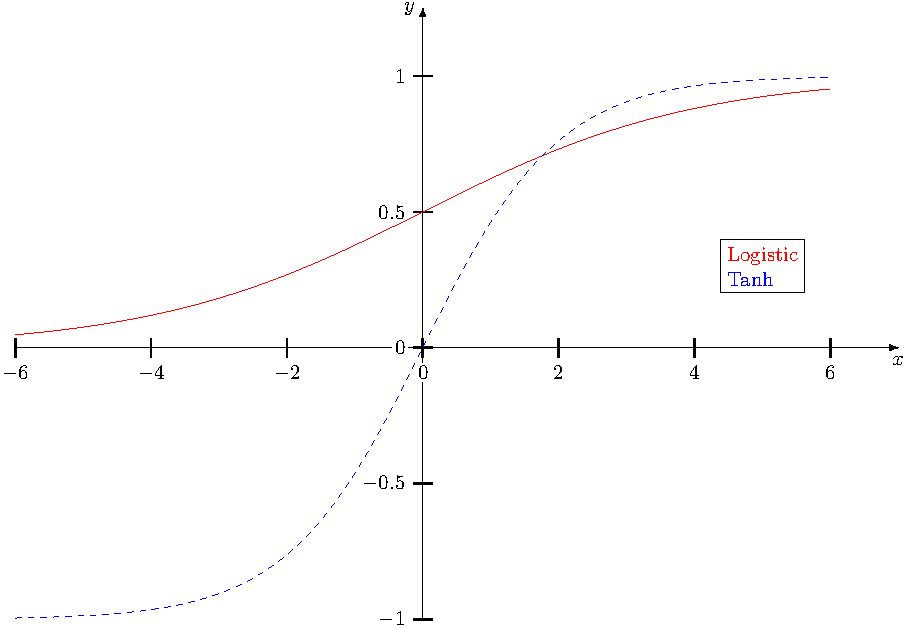
\includegraphics[width=0.4\linewidth]{2-1-1}
	}\hspace{0.1\linewidth}
	\subfigure[ReLU激活函数及其变体]{
		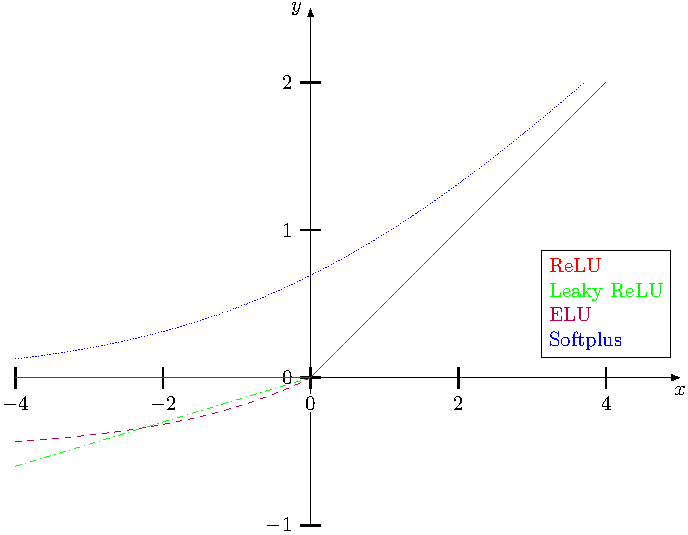
\includegraphics[width=0.4\linewidth]{2-1-2}
	}
	\caption{激活函数示意图} \label{fig:2-1} 
\end{figure}

图\ref{fig:2-1}中激活函数包括sigmoid、tanh、maxout、ReLU及其变体,例如leaky ReLU、ELU和PReLU等。输入卷积特征图的激活函数如下所示:
\begin{equation} \label{activation}
	T_l^k=f_A(F_l^k).
\end{equation}
其中$F_l^k$是卷积运算的输出,它通过激活函数$f_A(\cdot)$返回第$k$层的转换输出$T_l^k$。不同的激活函数用于引入特征的非线性组合。另外,ReLU及其变体的梯度有界,可以克服神经网络训练过程中梯度消失的问题。

批次归一化(Batch Normalization,BN)的提出是为了解决神经网络各层输出特征图内部协方差平移(Internal Covariate Shift,ICS)相关的问题。ICS偏移量导致各层输入分布与输出分布不一致,这会降低模型训练的收敛速度(通过将学习率强制为较小值来解决),并对参数初始化要求高。对变换后的特征图$T_l^k$执行批次归一化如下所示:
\begin{equation} \label{bn}
	N_l^k=\frac{F_l^k-\mu_B}{\sqrt{\sigma_B^2+\epsilon}}.
\end{equation}
其中$N_l^k$表示归一化特征图,$F_l^k$表示输入特征图,$\mu_B$和$\sigma_B^2$分别表示小批次特征图的均值和方差。批次归一化通过将特征图设为零均值和单位方差来统一其分布。此外,批次归一化可以平滑梯度流并充当调节因素,从而提高网络的泛化性。

Dropout引入了网络内部的正则化,在训练过程中它通过以一定概率丢弃神经元的方式提高网络的泛化性。在神经网络中,学习某个非线性组合会相互适应导致其过拟合。某些连接单元的这种随机丢弃会产生几种稀疏的网络体系结构,之后选择一个权重较小的代表性网络,将这种选择的架构视为所有提出网络的近似。

\subsubsection{深度卷积神经网络主要架构}
随着CNN成功应用于图像识别领域,Simonyan等人提出了模块化的分层结构体系VGG-19,如图\ref{fig:2-2}所示。与AlexNet相比,VGG的深度为$19$层,以模拟深度与网络表示能力的关系。VGG用一堆小尺寸的$3x3$卷积层代替了$5\times5$和$11\times11$卷积层,并通过实验证明,同时放置$3x3$卷积核可以达到大尺寸卷积核的效果。小尺寸卷积核的另一个好处是通过减少参数的数量降低了网络的计算复杂性。这些发现为在神经网络中使用较小尺寸的卷积核创造了新的研究趋势。虽然VGG未在2014年的ILSVRC竞赛中名列前茅,但由于其简单、同质的拓扑结构和增加的深度而闻名。VGG的不足之处主要在于计算成本高。即使使用小尺寸的卷积核,仍有约$1.4$亿个参数。
\begin{figure}[!hptb]
	\centering
	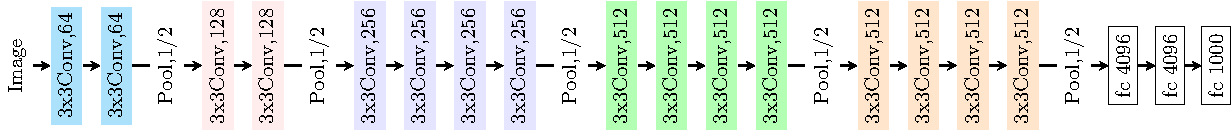
\includegraphics[width=\linewidth]{2-2}
	\caption{VGG16网络架构示意图}\label{fig:2-2}
\end{figure}

GoogleNet赢得了2014年ILSVRC竞赛的冠军,亦称为Inception-V1。GoogleNet体系结构的主要目标是在降低计算成本的同时实现高精度。它在卷积神经网络中引入了inception块的新概念,通过拆分、变换和合并的思想整合了多尺度卷积层。inception块的体系结构如图\ref{fig:2-3}所示。该模块封装了不同大小的卷积核($1\times1$、$3\times3$和$5\times5$),以捕获不同尺度(细粒度和粗粒度)的空间信息。GoogleNet有助于解决学习同一图像类别中存在的各种类型变体有关的问题。除了提高学习能力外,GoogleNet的优点还在于提高了CNN参数的利用率,以及应用批次归一化技术与RMSProp优化器加速其训练的过程。但是,GoogleNet的主要缺点是其异构拓扑结构需要在模块之间进行自定义。此外,GoogleNet的另一个限制是表示瓶颈,它极大地减少了下一层的特征空间,因此有时可能会导致有用信息的丢失。
\begin{figure}[!hptb]
	\centering
	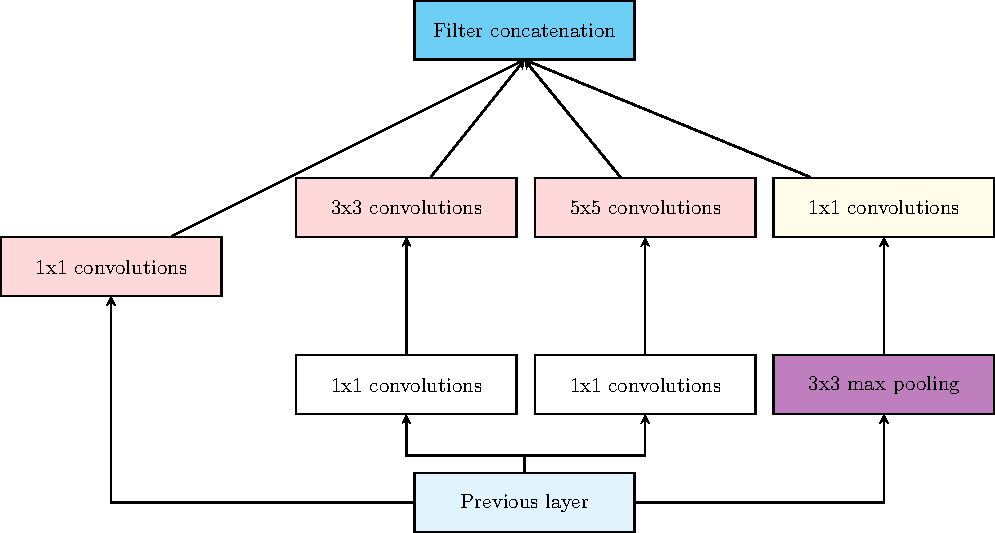
\includegraphics[width={0.8\linewidth}]{2-3}
	\caption{Inception块基本结构示意图}\label{fig:2-3}
\end{figure}

ResNet由He等人提出,被认为是深度网络的延续,其网络架构如图\ref{fig:2-4}所示。ResNet通过在卷积神经网络中引入残差学习的概念彻底改变了卷积神经网络架构,解决了神经网络训练过程中的退化问题。神经网络层数的加深致使神经网络参数空间变得复杂,因此提升了优化的难度。ResNet的残差结构有效降低了学习的难度,解决了深层神经网络的性能退化问题。
\begin{figure}[!hptb]
	\centering
	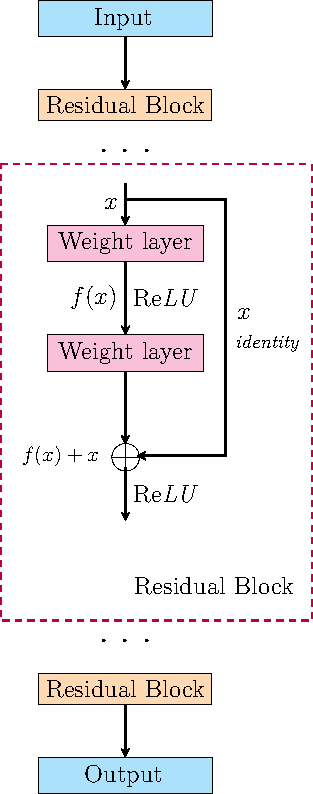
\includegraphics[height={0.6\linewidth}, width={0.3\linewidth}]{2-4}
	\caption{ResNet网络架构示意图}\label{fig:2-4}
\end{figure}

生成对抗网络(Generative Adversarial Networks,GAN)是Goodfellow等人开创性提出的一种生成式模型,其结构如图\ref{fig:2-5}所示。GAN一般由两个网络组成:生成器(Generator)和鉴别器(Discriminator)。其次,GAN是一种以半监督方式训练分类器的方法,用于解决带标签训练集样本少的问题。GAN模型训练时不像VAE一样需要对隐变量做出分布假设,生成器的参数更新不是直接来自数据样本,而是来自判别器提供的梯度信息。GAN本质上用判别器去学习损失函数,而非直接优化生成样本与标签的距离。
\begin{figure}[!htbp]
	\centering
	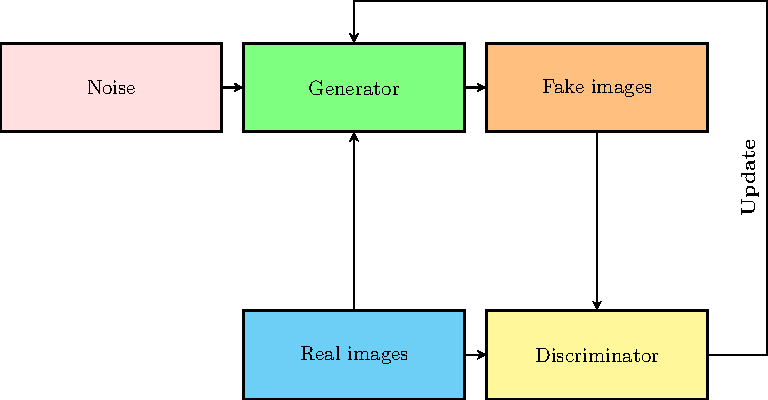
\includegraphics[width={0.8\linewidth}]{2-5}
	\caption{GAN网络架构示意图}\label{fig:2-5}
\end{figure}

GAN的学习优化过程就是一个极小极大博弈(Min-Max Game,MMG)问题,目的是寻找二者之间的一个纳什均衡,使生成器估计数据样本的真实分布。GAN的损失函数如下所示:
\begin{equation} \label{second:GAN}
	\min_{G}\max_{D}\quad V(D,G)=\mathbb{E}_{x\sim{p_{data}(x)}}[\log{D(x)}]+\mathbb{E}_{z\sim{p_{z}(z)}}[\log{(1-D(G(z)))}].
\end{equation}
在生成对抗网络中,如果没有对辨别器进行约束,那么其产生的梯度通常并不具有充分的信息来引导生成器进行更新,最新的解决方案是对判别器利用实谱归一化技术进行利普希茨约束。同时GAN生成的样本虽然具有多样性,但是存在模式崩溃与模式单一的现象。

U-Net由Ronneberger等人在Kaggle挑战赛上提出,它应用于医疗影像分割任务。U-Net是典型的Encoder-Decoder结构,Encoder进行特征提取,Decoder进行解码操作,如图\ref{fig:2-6}所示。
\begin{figure}[!htbp]
	\centering
	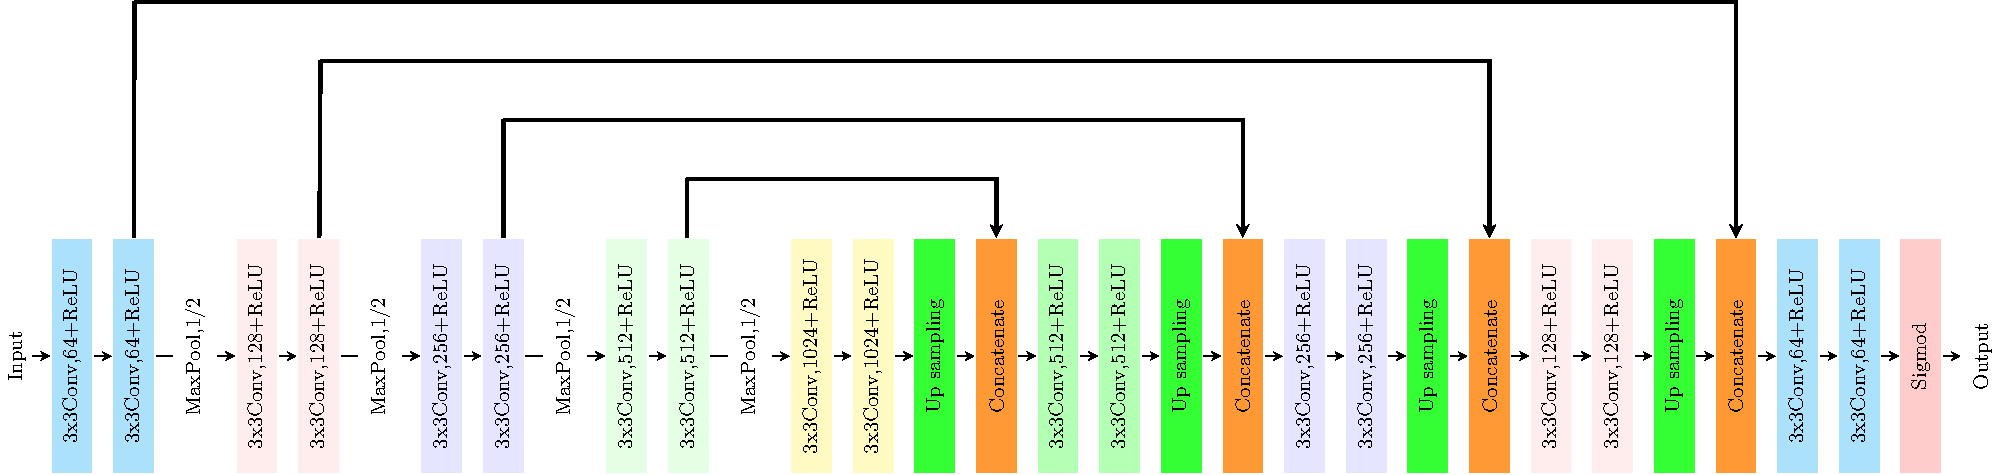
\includegraphics[width={\linewidth}]{2-6}
	\caption{U-net网络架构示意图}\label{fig:2-6}
\end{figure}

U-Net网络架构中一个重要的组成部分是在上采样中拼接了来自编码网络大量的浅层特征图,这些通道允许网络将上下文信息传播到具有更高分辨率的层。因此,拓展路径或多或少地与收缩路径对称,并产生一个U形结构。U-Net可以提取图像不同区域不同尺度的特征,这对像处理来说具有天然的优势。最近,U-Net结合循环神经网络(Recurrent Neural Network,RNN)、残差结构、注意力机制设计出R2U-Net、Deep Residual U-Net、Attention U-Net等语义分割网络,为自动驾驶、自动扣图等领域开辟出新的研究途径。

\subsection{基于深度学习的图像去噪算法}
深度学习技术在图像降噪方面获得了极大的成功。但是,处理不同类型噪声的学习方法存在较大的差异。具体来说,基于深度学习的方法可以有效估计真实的噪声分布\supercite{Chunwei}。但是,迄今为止很少有相关研究来总结用于图像去噪的不同深度学习技术。本节介绍了图像去噪领域内两种典型的深度学习去噪器DnCNN和IRCNN。

图像去噪任务要求在尽可能去除噪声的同时,还应保持图像的边缘、纹理等结构信息。再者,对于普遍存在的图像模糊问题,如何有效估计模糊过程、处理噪声和估计误差等,将对恢复高质量、清晰的图像至关重要。图像去噪任务的观测模型如下所示:
\begin{equation} \label{equation:2-6}
	y = x + v.
\end{equation}
其中$x,y,v$分别代表干净图像、噪声图像和高斯噪声(AWGN)。下面介绍两种经典的深度学习去噪模型:

(1)DnCNN由张凯等人提出,其网络架构如图\ref{fig:2-7}所示\supercite{Kai}。DnCNN采用残差学习训练残差映射$R(y)\approx{v}$,然后得到干净图像$x=y-R(y)$。DnCNN模型有两个主要特征:采用残差学习来学习$R(y)$,并结合BN层来加速训练过程;卷积与ReLU结合,DnCNN通过隐层逐渐将图像结构与噪声干扰分开。这种机制类似于EPLL和WNNM等方法中采用的迭代噪声消除策略,但DnCNN以端到端的方式进行训练。对于某一个特定的噪声水平,DnCNN可以在视觉效果和数值上达到当前SOTA的水平。再者,DnCNN可以扩展通用的降噪任务,即训练一个去盲高斯噪声的DnCNN模型可优于针对某种具体噪声水平的方法。同样的方法可以扩展到一般的降噪任务,例如单幅图像超分率和jpeg去块任务。
\begin{figure}[!htbp]
	\centering
	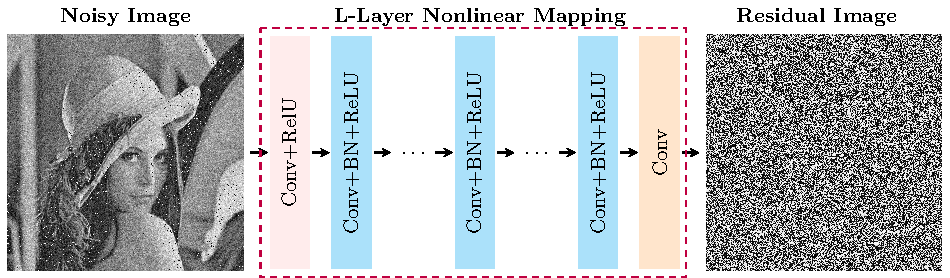
\includegraphics[width=\linewidth]{2-7}
	\caption{DnCNN网络架构示意图}\label{fig:2-7}
\end{figure}

(2)IRCNN同样由张凯等人提出,作为图像先验应用于去模糊、单幅图像超分辨率等图像反问题。其网络架构如图\ref{fig:2-8}所示\supercite{ZhangKai}。IRCNN使用空洞卷积扩大感受野以捕获更多的上下文信息。另外,空洞卷积不仅可以提高性能和效率,还能挖掘更多图像的边缘模式。在图像去噪任务中,背景信息对重构受损像素具有很大的作用。

一般用于扩大卷积神经网络感受野的方法为:一是增大卷积核尺寸;二是加深卷积深度。因此,最佳的设计是在现有卷积神经网络的结构体系之上,使用深度更深的$3\times3$卷积核。另外,扩张卷积以其扩大感受野的能力而闻名,同时保持传统$3\times3$卷积的优点。具有膨胀因子$s$的扩张卷积可简单地解释为大小为$(2s+1)\times(2s+1)$的稀疏滤波器,其中只有$9$个固定位置可以为非零数。因此,IRCNN每层的等效感受野是$3,5,7,9,7,5,3$,此时$L=7$,IRCNN网络的感受野是$33\times33$。如果使用传统的$3\times3$卷积核,网络感受野大小为$15\times15$或者具有相同感受野但深度为$16$。再者,DnCNN与IRCNN的去噪性能相近的情况下,对于不同输入尺寸的图像,使用空洞卷积的IRCNN测试速度优于DnCNN。
\begin{figure}[!htbp]
	\centering
	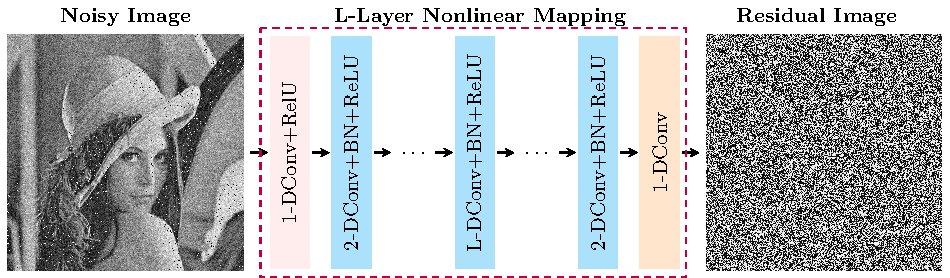
\includegraphics[width=\linewidth]{2-8}
	\caption{IRCNN网络架构示意图}\label{fig:2-8}
\end{figure}

\section{本章小结}
本章首先概述了非凸优化理论的基本问题与基本算法,其次介绍了深度学习领域的深度卷积神经网络结构与基于深度学习的图像去噪算法,最后给出了图像去噪领域中两种典型深度卷积神经网络去噪器DnCNN和IRCNN的网络架构。


